\chapter{Algebricks: A Data Model-Agnostic Compiler Backend}
\label{ch:algebricks}

In this chapter, we describe the design and implementation of the Algebricks layer. As we started to build the AQL compiler for the AsterixDB platform, we realized that having a generic compiler framework to compile declarative languages to evaluate using a parallel dataflow platform like Hyracks would be useful to the community at large. Based on prior research in the area of extensible systems and query algebras, we designed the Algebricks library to help query language implementors avoid spending time building a lot of boiler plate code that goes into implementing a full-fledged compiler. Algebricks, along with Hyracks, enables query language implementors to have a complete parallel query compiler in a matter of days.


\section{The Algebricks Framework}\label{sec:algebricks-fw}

Algebricks is an 
%data-model-agnostic, 
algebraic layer for parallel query
processing and optimization.
To be useful to implement various data-intensive query languages,
Algebricks has been carefully designed to be {\em agnostic} of the data model of the data that it processes. 
Logically, operators operate on collections of tuples containing data values. 
The types and formats of data values carried inside a tuple are not specified by the Algebricks toolkit; language implementors are free to define any value types as abstract data types. 
For example, a language developer implementing a SQL compiler on top of Algebricks would define SQL's scalar data types to be the data model, provide a type computer for SQL expressions, and implement runtime functions such as scalar functions and aggregate functions as well as runtime operations such as comparison and hashing. 
AQL~\cite{ASTERIX} has a richer set of data types, including various collection types and nested types, and these have been implemented on top of the Algebricks API
as well.

The Algebricks framework consists of the following parts:

%\begin{compactenum}
\begin{list}{\labelitemi}{\leftmargin=1em}\itemsep 0pt \parskip 0pt
\item A set of logical operators,
\item A set of physical operators,
\item A rewrite rule framework,
\item A set of generally applicable rewrite rules,
\item A metadata provider API that exposes metadata (catalog) information to Algebricks, and,
\item A mapping of physical operators to the runtime operators and connectors in Hyracks.
\end{list}
%\end{compactenum}

\begin{figure}[tb]
  \centering
  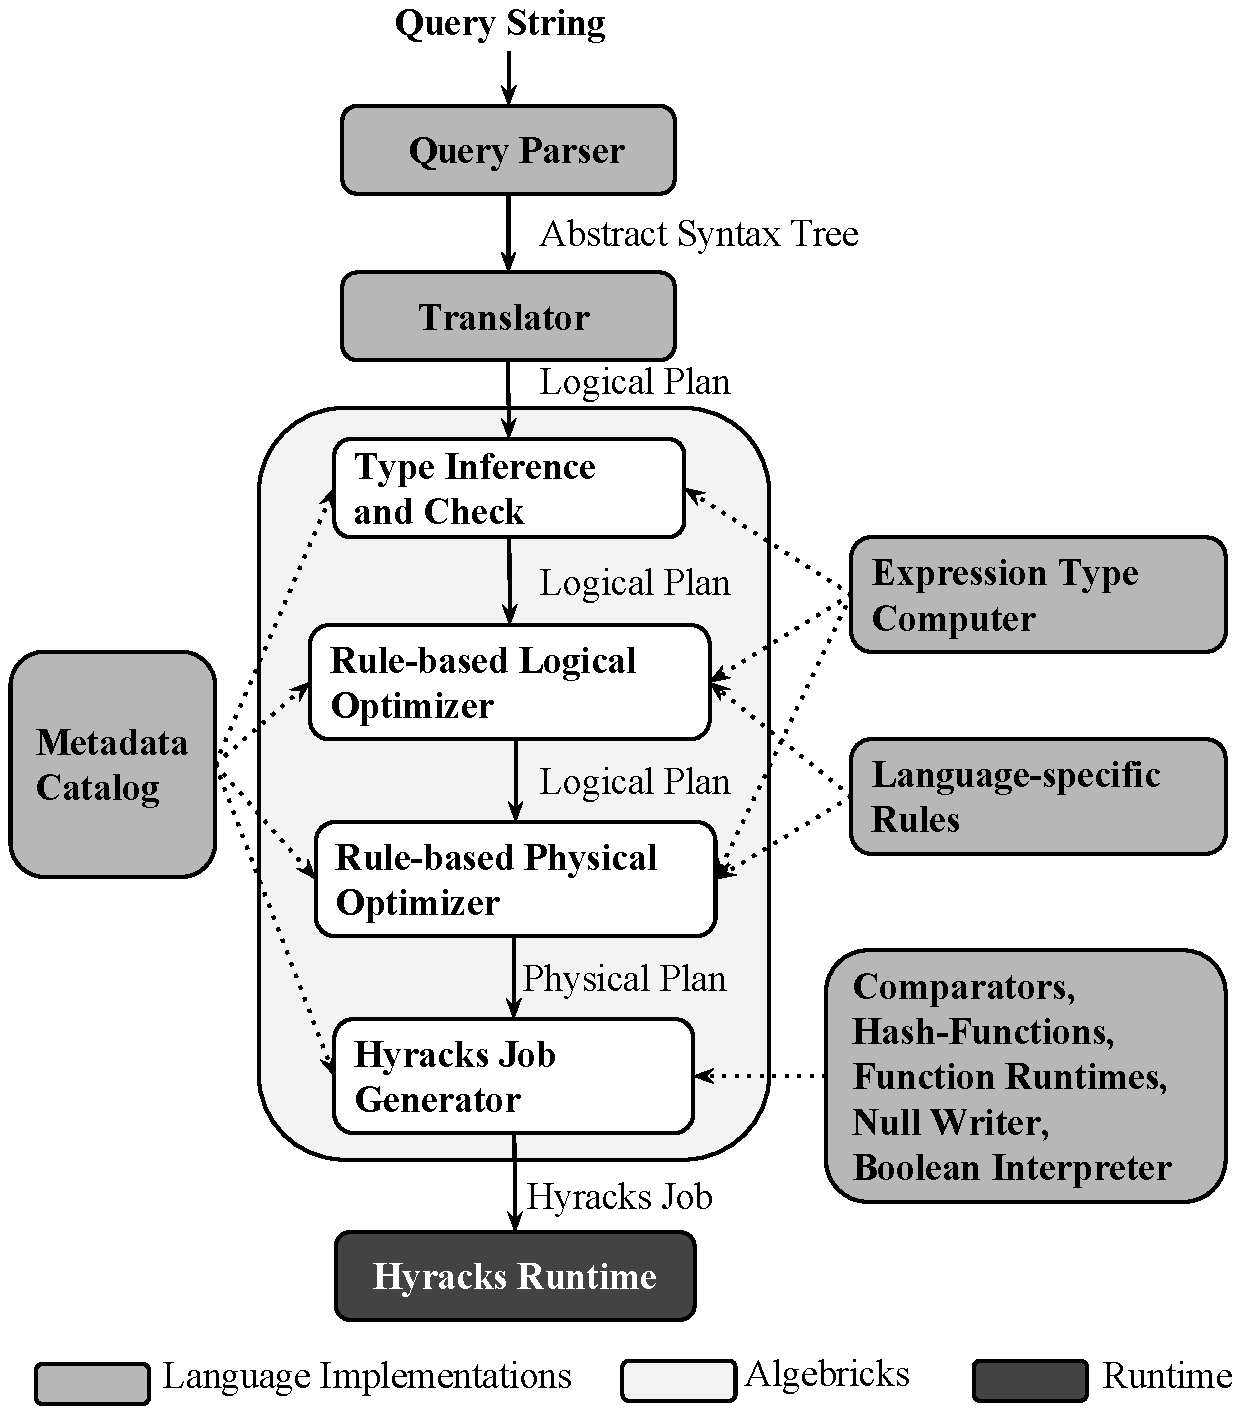
\includegraphics[width=5in]{images/compiler_flow}
  \vspace{-3ex}
  \caption{Flowchart of a typical Algebricks-based compiler.}
  \label{fig:flowchart}
\end{figure}

\textbf{Compilation Flow}. 
Figure~\ref{fig:flowchart} shows the typical sequence of compilation steps followed by a query processor built using Algebricks. 
An incoming query string is first lexically analyzed and parsed to construct an abstract syntax tree (AST).
This AST is then translated into 
the Algebricks logical plan, which is composed of logical operators (described in
Section~\ref{subsec:logoperators}) and serves as an intermediate representation to perform the next steps involved in query compilation. 
Type inference and checking is done over the initial logical plan, using a language-provided expression type computer which infers the type and checks type errors for each individual expression. 
The logical plan is then handed to the logical optimizer which rewrites it heuristically using logical rewrite rules. 
%The optimized logical plan is then translated to an Algebricks physical plan by selecting physical operators (described in
%section~\ref{subsec:phyoperators}) for every logical operation in the plan, by the physical optimizer. 
The physical optimizer translates the optimized logical plan to an Algebricks physical plan by selecting physical operators (described in
Section~\ref{subsec:phyoperators}) for every logical operation in the plan.
Both optimizers are rule-based and configured by selecting the set of rules to execute during the optimization phases.
The resulting physical plan is processed by the Hyracks Job Generator to produce a Hyracks job that is parallelized and evaluated by the Hyracks
execution engine.

\textbf{Rewriting Rules}. 
The query parser and translator (the first two stages in Figure~\ref{fig:flowchart} are query language specific and must be implemented by a query language developer. 
The next three stages (the optimizers and Hyracks job generator) are provided by the Algebricks library to be used by the developer. 
Algebricks also includes a library of language-agnostic rewrite rules that can be reused by the compiler developer. 
Additional language-specific rules are usually required in the optimization process, too. 
%VASSILIS Check
These need to be implemented by the developer by extending well-defined interfaces in the Algebricks library.
Note that a language-provided expression type computer should be called during certain rule applications to propagate updated types for the updated intermediate logical plans. 
The rewrite rule framework is described in Section~\ref{subsec:rewriter}.

\textbf{Metadata Catalog}. As shown in Figure~\ref{fig:flowchart}, the various phases of the query compilation process need access to information about the
environment in which the query is being compiled (usually described as catalog metadata). 
%The catalog contains metadata about data sources that are accessible in a query. 
The catalog is the authoritative source of logical properties of sources (such as schema,
integrity constraints, key information, etc.) and their physical properties (access methods, physical location, etc.) Algebricks
provides a Metadata Interface (Section~\ref{subsec:metadata}) that must be implemented by the compiler developer so that the various parts of the Algebricks
compiler can access relevant metadata information. 
%The Metadata Interface is described in Section~\ref{subsec:metadata}.

\textbf{Runtime Operations/Functions}. 
The Hyracks Job Generator maps physical operators selected by the Physical Optimizer to Hyracks runtime operators and connectors. 
In the process of this translation, the runtime operators need to be injected with data model-specific operations. 
The exact nature of the operation depends on the runtime operator being used. 
For example, the Sort operator  must be provided a comparator to compare two data model instances so that the input records can be sorted; the  Hash-Join operator needs a hash-function and a comparator to compute its result; the Select operator requires a boolean interpreter to interpret the result of its filtering condition expression; the Outer-Join operators need a null writer to generate null fields according to the language-defined data format. 
When using Algebricks, the language developer must provide families of operations (usually one family for each data type, for example, comparators and hash functions) that are needed for correct runtime Job construction.
Finally, the language developer must implement a mapping from function expressions to its own function runtime implementations (e.g., arithmetic functions, string functions, aggregate function, etc.) so that the data model agnostic runtime operators (e.g., select, assign, aggregate, etc.) can evaluate the data model-dependent functions.



\subsection{Metadata Interface}\label{subsec:metadata}

Every data-management system that accesses stored data or external data sources to process queries requires some form of metadata that describes locations of the stored files or external data sources and the various access paths available to get to the data bits. 
For example, relational databases use a catalog to store information (schema) about
the tables and indexes present in the database; such information is used by the query compiler when compiling query plans. 
Algebricks provides a Metadata Interface which must be implemented by the author of the host language so that the Algebricks compiler can access metadata information required during the compilation process. 
The goal of this interface is to allow Algebricks access to all relevant details about datasources while not constraining the host language to a specific representation of the metadata internally.
%
The Metadata Interface provides the following pieces of information to the compiler:

\begin{asparaitem}
\item \textbf{Data Source Metadata}. Stored collections of data or external data sources are both modeled as a Data Source in Algebricks. 
For example, in HiveQL, a table would be considered a Data Source while a dataset or an external data feed would be modeled as a Data Source in AsterixDB~\cite{ASTERIX,DBLP:conf/edbt/GroverC15}.
The Data Source interface enables Algebricks to get metadata about the data that it represents. 
Source metadata can be broadly classified as Logical Metadata and Physical Metadata. 
Logical Metadata about a Data Source includes the type information of the data it represents and other logical properties such as functional dependencies and integrity constraints (keys, etc.). 
Physical Metadata provides details of how the data is physically stored or obtained, specifically providing partitioning information and any local ordering present in the stored data.

\item \textbf{Access Path Binding}. The Metadata Interface in Algebricks also serves as a factory to create the runtime binding to connect the compiled Hyracks job to the ``last mile" (operators that are capable of reading the data from the stored location).

\item \textbf{Function Metadata}. Algebricks further uses the Metadata Interface to find Function Metadata to optimize function applications that appear in the plan being compiled.
\end{asparaitem}

\subsection{Logical Operators}\label{subsec:logoperators}

The logical operators in Algebricks draw inspiration from a variety of algebraic systems proposed for nested-relational models description
\cite{Jaeschke:1982:RAN:588111.588133,NST-Algebra} and for the processing of semi-structured data \cite{Papakonstantinou2003299,Jagadish:2002gu,Deutsch:2004:NFL:1316689.1316706}. 
Tuples in Algebricks are used as an abstraction that hold values.
Algebricks operators logically consume and produce collections of tuples. 
Tuples contain fields that are created and manipulated by the operators; 
field names are represented by names prepended with a \$ sign in the description that follows. 
Note that tuples as used in this section are not to be confused with tuples in the relational model, as Algebricks tuple field
values are allowed to be of arbitrary data types (not just scalar types like in the relational model). 
For example, in AsterixDB, an entire record (a composite data structure that contains name-value pairs) can be the value of a field in an Algebricks tuple and a concrete field type (i.e., open type in AQL~\cite{ASTERIX}) can even be determined at runtime.
\eat{\nick{I didn't fully understand the difference between tuples in Algebricks and in the relational model. Is it just that we allow nesting? Then we could say it is similar to nested relational datamodels or maybe to query languages with complex values. These are all well known concepts.}}

Operators may also contain references to scalar or aggregation functions wrapped inside a generic logical expression interface which exposes the used fields and allows for field name substitution. 
This allows Algebricks to rewrite the plan, while at runtime native functions are run against the data model of the implemented language.
A logical expression also has methods for computing logical constraints that can be inferred from that expression.
The constraints currently implemented are functional dependencies and equivalence classes.
They are used during rewriting, e.g. to reason about interesting orders and partitioning properties.
There are three implementations of the logical expression interface:
\eat{
\nick{The part about ILogicalExpression looks like it hasn't been integrated
it (probably my fault :-) It could have its own paragraph title, so it
stands out as a sub-topic. And rephrase the glue text to say more
clearly that we isolate everything related to scalars in these
ILogicalExpression instances.}
}

\begin{list}{\labelitemi}{\leftmargin=1em}\itemsep 0pt \parskip 0pt
\item {\em Constant} holds constant values.
\item {\em VariableReference} points to a logical variable (with a logical id) which is a column in a tuple.
\item {\em FunctionCall} holds a function identifier and references to argument expressions.
  It models all expressions which are not constants nor variables and it is the only kind of expression that is not a leaf in an expression tree.
\end{list}

{\em FunctionCall} is further refined by four implementations:

\begin{list}{\labelitemi}{\leftmargin=1em}\itemsep 0pt \parskip 0pt
\item {\em ScalarFunctionCall} is used for functions that compute their result by looking at only one tuple.

\item {\em AggregateFunctionCall} functions produce a result after iterating over a collection of tuples.
SQL aggregate functions belong here.
%fall in this category.

\item {\em StatefulFunctionCall} is similar to AggregateFunctionCall, but produces a result after each tuple, not only at the end. 
      Position variables in XQuery fall in this category: for every binding in a for-clause, they output the binding's index in the sequence.

\item {\em UnnestingFunctionCall} is given an input tuple and then can be called multiple times, each time returning a possibly different result, until a special value is returned. 
      Examples are the {\em range} function in Asterix which returns integer values from a specified range or the {\em collection} function in XQuery which returns nodes according to the arguments' available collection.
\end{list}

From a given function expression, a query language implementation can create the runtime artifact, i.e., an evaluator, 
which is capable of implementing its language-specific runtime semantics.
Evaluators run code specific to every language: in the case of Hivesterix (a HiveQL implementation on top of Algebricks; see Section~\ref{sec:hivesterix}), it runs the native Hive evaluators, which were not designed specifically for Algebricks. 
  Translation between logical function calls and evaluators is done at job generation time (Section~\ref{subsec:jobgen}). 
  This design has the advantage that it allows multiples ways of implementing the translation from logical to physical.
  In Hivesterix, this is done by having the function call expressions reference their evaluators.
  In AsterixDB, evaluators register themselves in a global map which is keyed on function identifiers.


\subsection{Physical Operators}\label{subsec:phyoperators}

While the logical operators described in Section~\ref{subsec:logoperators} capture the semantics of an Algebricks logical plan, physical operators are used to specify the exact algorithm to use for evaluating each operator. 
During the query rewrite process (described in Section~\ref{subsec:rewriter}) rules assign physical operators to each logical operator in the query plan, thus deciding the concrete algorithms to use in evaluating the query. 
Most logical operators in Algebricks map to a unique physical operator. 
However, Join and Group-By operators have multiple concrete implementations. Physically, joins can be performed using the Hybrid-Hash Join~\cite{DeWitt:1984:ITM:602259.602261} or the Nested-Loop Join algorithms. 
The Group-By operation can be performed using a pre-clustered implementation that assumes that its input is already clustered with respect to the 
grouping keys or by using a hash-based or sort-based Group-By algorithm that is capable of spilling to disk when the in-memory state exceeds available memory \cite{WenBCT13}.

In addition to physical operators corresponding to logical operators, Algebricks also provides physical operators to enforce order properties as well as partitioning properties of data distributed to individual operations during parallel evaluation of the query. 
Data distribution between operator partitions is expressed using an Exchange operator, motivated by~\cite{exchange}. 
\eat{\nick{It is true we use Exchange operators to enforce partition properties.
But Sort may also be used as an enforcer (for order properties), even
if the query semantics doesn't require sorting. In case we don't have
it somewhere else, we could add a short sentence saying we can
introduce enforcers for local properties (ordering and grouping).
 }
}
Currently, the data distribution strategies offered by Exchange operators in Algebricks are:

\begin{asparaitem}

\item {\em One-to-One Exchange}: This strategy is used for the local movement of data without redistribution of
data between partitions.

\item {\em Hash Exchange}: The Hash Exchange strategy hashes specified fields to determine how tuples are to be routed to the destination
partitions. This operator helps in partitioning data based on field values so that two tuples with the same partitioning field
values are routed to the same destination.

\item {\em Range Exchange}: The Range Exchange strategy uses a provided range vector to determine the destination partition to send a record to, based on the values of specified fields. 
The range vector maps disjoint ranges of values to target partitions. The value of the partitioning fields of each record are used to probe the range vector to decide the target partition. 
In addition to sending equal values to the same partition, range-based partitioning also sends close-by values to the same site. 
Such a distribution strategy is useful for performing a global sort in a parallel manner.

\item {\em Random Exchange}: Sometimes it is desirable to redistribute data to a set of partitions in a load-balanced manner, but without necessarily maintaining a value-based partitioning property. 
The Random Exchange Operator does exactly that by sending each record to a randomly determined partition.

\item {\em Broadcast Exchange}: The Broadcast Exchange strategy is used to make sure that the same data is delivered to every partition of the next operator. 
An example situation for the use of the Broadcast Exchange operator is while joining a small relation with a large partitioned relation. 
The small relation is broadcast to each machine where a partition of the large relation resides prior to performing a local join at each site.

\end{asparaitem}


%In addition to the data-exchange strategies listed above, 
Moreover, the Hash Exchange, Range Exchange, and Random Exchange strategies have a second variant each, namely, Hash-Merge Exchange, Range-Merge Exchange, and Random-Merge Exchange. A merge variant applies the same partitioning strategy as the non-merge variant, but uses a priority queue on the receiving side that merges all incoming streams so as to maintain a specified sort order that the data originally possessed before partitioning. 



\eat{
Table~\ref{tbl:phyoperators} summarizes the available
Physical Operators in Algebricks.

\begin{center}
\begin{table*}[ht]
{\small
\hfill{}
\begin{tabular}{ | l | l | p{3in} | }
\hline
Logical Operator & Physical Operator(s) & Description \\

\hline

\multirow{2}{*}{GroupBy Operator} & Presorted GroupBy & \\
\cline{2-3}
 & External Hash-Sort GroupBy & \\
\hline
\multirow{3}{*}{Join Operator} & Grace-Hash Join Operator & \\
\cline{2-3}
 & Hybrid-Hash Join & \\
\cline{2-3}
 & Nested-Loop Join & \\
\hline
\multirow{8}{*}{Exchange Operator} & One-to-One Exchange & \\
\cline{2-3}
 & Hash-Partition Exchange & \\
\cline{2-3}
 & Range-Partition Exchange & \\
\cline{2-3}
 & Random Exchange & \\
\cline{2-3}
 & Hash-Partition-Merge Exchange & \\
\cline{2-3}
 & Range-Partition-Merge Exchange & \\
\cline{2-3}
 & Random-Merge Exchange & \\
\cline{2-3}
 & Broadcast Exchange & \\
\hline
\end{tabular}
\caption{Algebricks Physical Operators}
\label{tbl:phyoperators}
}
\end{table*}
\end{center}
}

In Algebricks, the physical operator layer is extensible.
Compilers on top of Algebricks can register new physical operators by implementing the following interface:

\begin{java}
public interface IPhysicalOperator {
    public PhysicalRequirements requiredPropertiesForChildren(
        IPhysicalPropertiesVector requiredByParent);

    public void deliveredProperties(ILogicalOperator op,
        IOptimizationContext context);

    public void contributeRuntimeOperator(
        IHyracksJobBuilder builder,
        IOpSchema propagatedSchema, IOpSchema[] inputSchemas,
        IOpSchema outerPlanSchema);
}
\end{java}


The methods \codepiece{requiredPropertiesForChildren} and \codepiece{deliveredProperties} compute and propagate ordering, grouping and partitioning properties, close in spirit to SCOPE~\cite{ScopeJournal}.
These properties guarantee that the correct semantics of the operators are implemented, e.g., a Pre-Clustered Group-By will have its inputs partitioned by (a subset of) the group-by key and locally clustered on each partition, while allowing for optimizations, e.g., if the data partitioning already satisfies the requirements, no re-partitioning of the input is needed.
The \codepiece{contributeRuntimeOperator} method is essential in the job generation phase, discussed in Section~\ref{subsec:jobgen}.

In AsterixDB, we need physical operators for B-tree indexes, to enable efficient access to the native storage layer~\cite{storage}. 
Since they are AsterixDB specific, they cannot be part of the Algebricks library, so they are added as language specific operators for accessing its native storage layer~\cite{storage}.
%, including B-tree indexes, which are not part of the Algebricks library. 
The BTreeSearch physical operator's \codepiece{contributeRuntimeOperator} constructs a Hyracks B-Tree search runtime operator which is added to the job DAG together with an incoming edge from the Hyracks operator that produces the search intervals. 
BTreeSearch generally delivers a local ordering property on the key fields. For a primary index, the operator also delivers a hash-partitioning property of the key fields.
The operator generally requires its input (a stream of key intervals) be broadcast over the locations where the index is partitioned, but for primary indexes, the required property is hash-partitioning.

\eat{
If the output of the BTreeSearch operator is used by a join, \codepiece{requiredPropertiesForChildren} will generally have a broadcast requirement, but for an equality search on a primary index, this can be replaced by hash partitioning. 
Also, in the case of a primary index, the physical requirements contain a local order on the search keys so the B-tree search is more efficient.
}

\subsection{Rewriter}\label{subsec:rewriter}

The Algebricks optimizer uses Logical-to-Logical rewrite rules to create alternate logical formulations of the initial DAG.
Logical-to-Physical rewrite rules then generate a DAG of physical operators that specify the algorithms to use to evaluate the query.  
For example, a Join operator might be rewritten to a Hash-Join
physical operator. 
We expect that most language implementors using Algebricks will need a rewriting framework to perform additional useful data model-specific optimizations.
The Algebricks toolkit contains a rewriting framework that allows users to write their own rewrite rules, but it also comes with a number of ``out of the box'' rules that the user can choose to reuse for compiling their high-level language.
Examples of rules that apply for most languages include:

\begin{asparaitem}
\item {\bf Push Selects}: Rule for pushing filters lower in the plan to eliminate data that is not useful to the query.
\item {\bf Introducing Projects}: Rule to limit the width of intermediate tuples by eliminating values that are no longer needed
in the plan.
\item {\bf Query Decorrelation}: Rule to decorrelate nested queries to use joins when possible.
\end{asparaitem}

An example rule implemented in AsterixDB that is not of general applicability is one that uses ASTERIX metadata~\cite{ASTERIX} to determine if a field is present in the declared schema (i.e., if its presence is known a priori) in order to determine which field access method to use: field-access-by-index or field-access-by-name.

The rewriter uses the properties below, which, together with the graph of operators, dictate whether a rule is fired or not.
%Those properties include:

\begin{list}{\labelitemi}{\leftmargin=1em}\itemsep 0pt \parskip 0pt
\item {\bf Used/Produced Variables}. Operators schemas determine how projections and selections
are pushed and are needed by most rules that change the order of operators.

\item {\bf Functional Dependencies and Data Properties}. The process of rewriting into a physical DAG uses partitioning properties and local physical properties (grouping, ordering) of input data sources. 
Similar to SCOPE~\cite{ScopeJournal}, these are computed based on functional dependencies and variable equivalence classes.
Based on partitioning properties, Data Exchange operators~\cite{Dewitt:1990fk,journals/tkde/Graefe94} are introduced
to perform data redistribution between partitions.

\item {\bf Equivalence Classes}. The optimizer analyzes equivalence classes of variables.
%Variables within an equivalent class are equivalent to each other.
For example, after an equal inner join, a variable in the left-hand side join key
and its corresponding variable in the right-hand side join key are equivalent after the join operator. 
With the information of equivalent classes, functional dependencies and data properties are further propagated.
\end{list}

\subsection{Job Generation}\label{subsec:jobgen}

The job generation component outputs a Hyracks job implementing the Algebricks plan (Figure~\ref{fig:flowchart}).
The job is constructed by walking the plan and calling the \codepiece{contributeRuntimeOperator} method on the physical operators.
A physical operator can contribute either
\begin{inparaenum}[(a)]
  \item a full Hyracks operator,
  \item a micro-operator, which becomes part of a pipeline running inside one Hyracks operator,
  \item a connector, typically when the Algebricks operator is an exchange.
\end{inparaenum}
The Hyracks runtime for \codepiece{DataSourceScan} and 
\codepiece{WriteResult} operators are obtained through the Metadata Interface which also returns partitioning information needed to instantiate those operators. 
%In the case of sorting or join operators that need hash functions or comparators, they are picked based on the field types and set in the corresponding Hyracks operators.
%\nick{Is it still 1-to-1 between Algebricks plan and Hyracks job or could we generate multiple jobs to implement a plan?}
While the job generator currently only generates Hyracks jobs, its architecture conceptually supports other runtimes (e.g. Spark, Tez).
E.g., instead of generating Hyracks connectors, in Tez we would create ``edges" and in Spark ``partitioners", which are all similar concepts representing data movement from producers to consumers.


\section{Using Algebricks}
\label{sec:usage}

In this section we delve into the details of how three query processing systems --- Hivesterix (Hive-on-Hyracks), AsterixDB, and VXQuery --- use Algebricks to compile queries.

\subsection{Hivesterix}
\label{sec:hivesterix}
Hivesterix compiles HiveQL queries to run on the Hyracks platform.
For each HiveQL query, 
Hivesterix obtains the physical query plan from the Hive compiler
and turns that into an Algebricks logical plan for
Algebricks to produce a Hyracks job that calls
back to Hive's function evaluators at runtime.
Let us walk through a HiveQL example.
A simple HiveQL query shown below filters records from a TPC-H ``lineitem'' table to retain only those records which satisfy the filter predicate. 
Furthermore, the aggregated overall ``revenue" from selected records are returned. 
The ``lineitem'' table used in the query has the schema shown in Table~\ref{tbl:lineitemchema}. 

%\nick{The faded colored boxes for logical plans are not easy to read. Could we use something similar to the ones for the Hyracks jobs, even if just one box?}
\lstset{numbers=left, numberstyle=\tiny, stepnumber=1, numbersep=5pt}
\begin{center}
\scriptsize
\begin{lstlisting}
select sum(l_extendedprice*l_discount) as revenue
from lineitem
where l_shipdate >= '1994-01-01'
  and l_shipdate < '1995-01-01'
  and l_discount >= 0.05 and l_discount <= 0.07
  and l_quantity < 24;
\end{lstlisting}
\end{center}


Hivesterix translates this query into the Algebricks plan below. In the plan, ``algebricks-*" (e.g., algebricks-gte, algebricks-lte) is a function
that Algebricks can recognize during rewriting but will use a language-provided runtime implementation at evaluation time.

% TODO should this be vertical table instead of horizontal?
\begin{table*}
\tiny
\begin{center}
\begin{tabular}{|l|l|l|l|l|l|l|l|l|}
\hline
Column Name &  l\_orderkey & l\_partkey & l\_suppkey & l\_linenumber & l\_quantity & l\_extendedprice & l\_discount & l\_tax\\ 
\hline
Data Type & bigint & bigint & bigint & bigint & float & float & float & float\\
\hline
\hline
Column Name & l\_returnflag & l\_linestatus & l\_shipdate & l\_commitdate & l\_receiptdate &l\_shipinstruct & l\_shipmode & l\_comment\\
\hline
Data Type & string & string & string & string & float & float & string & string\\
\hline
\end{tabular}
\caption{Schema of the TPC-H lineitem table.}\label{tbl:lineitemchema}
\end{center}
\end{table*}


\eat{
\begin{table}[!ht]
\begin{center}
\begin{tabular}{|l|l|}
\hline
Column Name & Data Type \\
\hline
\hline
l\_orderkey & bigint \\
\hline
l\_partkey & bigint \\
\hline
l\_suppkey & bigint \\
\hline
l\_linenumber & bigint \\
\hline
l\_quantity & float \\
\hline
l\_extendedprice & float \\
\hline
l\_discount & float \\
\hline
l\_tax & float \\ 
\hline
l\_returnflag & string \\
\hline
l\_linestatus & string \\
\hline
l\_shipdate & string \\
\hline
l\_commitdate & string \\
\hline
l\_receiptdate & float \\
\hline
l\_shipinstruct & float \\
\hline
l\_shipmode & string \\
\hline
l\_comment & string \\
\hline
\end{tabular}
\caption{Schema of the TPC-H lineitem table.}\label{tbl:lineitemchema}
\end{center}
\end{table}
}

\begin{center}
\scriptsize
\begin{lstlisting}
WRITE_RESULT( $$revenue )
AGGREGATE( $$revenue:sum($$l_extendedprice*$$l_discount) )
SELECT( algebricks-and(
    algebricks-gte($$1_shipdate, '1994-01-01'),
    algebricks-lt($$1_shipdate, '1995-01-01'),
    algebricks-gte($$l_discount, 0.05),
    algebricks-lte($$l_discount, 0.07),
    algebricks-lt($$l_quantity, 24)) )
ASSIGN( $$l_shipdate, $$l_discount, $$l_extendedprice, 
    $$l_quantity:
    column_expr($l, "l_shipdate"),
    column_expr($l,"l_discount"),
    column_expr($l, "l_extendedprice"),
    column_expr($l,"l_quantity") )
UNNEST( $$l:dataset(lineitem) )
EMPTY_TUPLE_SOURCE
\end{lstlisting}
\end{center}

While reading Algebricks plans, it is important to note that the dataflow is assumed to flow from the bottom of the plan to the top. 
The ``unnest'' operator produces the tuple streams from rows in the ``lineitem'' table. 
The Metadata Interface (Section~\ref{subsec:metadata}) implemented in Hivesterix probes the Hive meta-store (the catalog database used by Hive-on-Hadoop) to get schema information about the table accessed by the query. 
As seen in Table~\ref{tbl:lineitemchema}, the ``lineitem'' table has sixteen columns. 
Note that the translator does not prune the source fields not used in the query.  
Algebricks includes the logic necessary to perform this pruning. 
Continuing on with the initial plan for the query, the translator creates an ``assign" operator to extract fields from input tuples and a ``select'' operator to represent the ``where'' clause in the query. 
Finally, the ``aggregate'' operator is used to perform the aggregate sum and a ``write'' operator is used to write the results to HDFS. 
%Readers will find this expression of the query reminiscent of relational algebra~\cite{relalgebra} expressions.

After the translated plan is constructed, Hivesterix proceeds to optimize the query.
The Hivesterix optimizer is populated with a total of 61 optimization rules out of which 4 rules are specific to Hivesterix and the rest are part of the common Algebricks framework. 
Figure~\ref{fig:hivestrix_hyracks_job} visualizes the finally generated Hyracks job from the optimizer.
The Algebricks rewrite rules have all the logic necessary to parallelize the query without the need for Hivesterix to provide any additional code. 


\begin{figure}[!ht]
\vspace{-.8ex}
\centering
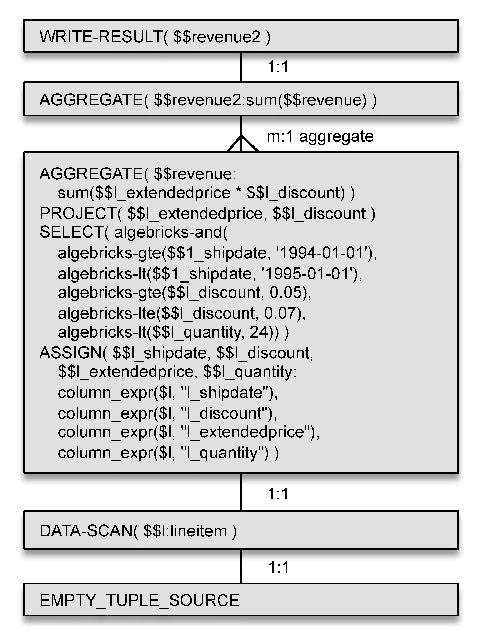
\includegraphics[width=0.70\columnwidth]{images/hivestrix_hyracks_job}
\vspace{-1ex}
\caption{Hivesterix Hyracks Job.}
\vspace{-.8ex}
\label{fig:hivestrix_hyracks_job}
\end{figure}


\eat{
\begin{center}
\scriptsize
\begin{lstlisting}
WRITE_RESULT( $$revenue2 )
ONE-TO-ONE EXCHANGE
AGGREGATE( $$revenue2:sum($$revenue) )
M-TO-ONE EXCHANGE
AGGREGATE( $$revenue:sum($$l_extendedprice*$$l_discount) )
ONE-TO-ONE
PROJECT( $$l_extendedprice, $$l_discount )
ONE-TO-ONE EXCHANGE
SELECT( algebricks-and(
    algebricks-gte($$1_shipdate, '1994-01-01'),
    algebricks-lt($$1_shipdate, '1995-01-01'),
    algebricks-gte($$l_discount, 0.05),
    algebricks-lte($$l_discount, 0.07),
    algebricks-lt($$l_quantity, 24)) )
ONE-TO-ONE EXCHANGE
ASSIGN( $$l_shipdate, $$l_discount, $$l_extendedprice,
    $$l_quantity:
    column_expr($l, "l_shipdate"),
    column_expr($l, "l_discount"),
    column_expr($l, "l_extendedprice"),
    column_expr($l, "l_quantity") )
ONE-TO-ONE EXCHANGE
DATA-SCAN( $$l:lineitem )
EMPTY_TUPLE_SOURCE
\end{lstlisting}
\end{center}
}

Note that most of the final Hyracks job looks similar to the original translated plan with the following differences:

\begin{list}{\labelitemi}{\leftmargin=1em}\itemsep 0pt \parskip 0pt
\item A project operator is injected into the plan to prune unnecessary columns.
\item An additional aggregate operator is injected to perform local aggregate in order to save the network bandwidth consumption, since the aggregation
function \textit{sum} is distributive.
\item An exchange operator with the associated data redistribution strategy has been introduced between every pair of operators. 
Operators below the lower aggregate operator use only one-to-one exchange operators.  
A m-to-one exchange is placed between the lower (local) aggregate and the higher (global) aggregate.
\end{list}



\subsection{Apache AsterixDB}

\eat{
\begin{itemize}
\item Very brief description of AsterixDB (one Paragraph)
\item Description of the datasets \& showing sample records 
\item Description of the query (in plain English)
\item Putting references to logical, optimized logical and physical plans
\item Describing the Hyracks job in details (broken into multiple phases): pushing selections down for each dataset, the intermediate partitioning step prior to the join, the HHJ step (AsterixDB uses HHJ for equi-joins), final record-construction step and results distribution)
\item Highlight and emphasize on the functions, rules and parts that fully reside in the AsterixDB code base (not part of the Algebricks) to clarify which parts are (re)-used from the Algebricks framework
\end{itemize}
}

Apache AsterixDB is a full-featured Big Data Management System for managing large quantities of semi-structured data. It is currently undergoing incubation at the Apache Software Foundation (ASF). 
AsterixDB's data model supports JSON-like data and adds more primitive and structured data types to JSON's data types.

As a slightly more complex example, consider the query below in the Asterix Query Language (AQL)~\cite{ASTERIX}.
This query performs a join between two natively stored data collections, ``GleambookMessages'' and ``GleambookUsers'',
that matches records from the two datasets on the ``author\_id'' and ``id'' fields respectively. Note that as allowed by the flexible AsterixDB data model,
``author\_id'' is not in the declared schema of ``GleambookMessages''
but ``id'' is part of the ``GleambookUsers'' schema.
Furthermore, we limit the results to contain users whose ``user\_since'' is within a time range and messages whose ``send\_time'' is within a specific time interval. Results are in the form of ADM (Asterix Data Model)~\cite{ASTERIX} records with two attributes, ``uname'' and ``message''. 

\begin{center}
\scriptsize
\begin{lstlisting}
for $message in dataset GleambookMessages
for $user in dataset GleambookUsers
where $message.author_id = $user.id 
  and $user.user_since >= datetime('2008-10-24T14:21:21')
  and $user.user_since < datetime('2008-10-25T14:21:21')
  and $message.send_time >=datetime('2011-02-24T20:01:48')
  and $message.send_time < datetime('2011-02-25T05:01:48')
return {"uname": $user.name, "message": $message.message}
\end{lstlisting}
\end{center}



\eat{
\begin{center}
\scriptsize
\begin{lstlisting}
{"message_id": int64("1"),
"author_id": int64("1"), 
"in_response_to": int64("33331"),
"sender_location": point("32.19,70.92"),
"send_time": datetime("2011-06-06T09:42:22"),
"message": "love samsung the screen is awesome"}

{"id": int64("1"),
"alias": "Chastity0001",
"name": "ChastityCarden",
"user_since": datetime("2010-05-07T19:13:33"),
"friend_ids":
 {{int64("2818"), int64("6982"), int64("13039")}}, 
"employment": [{"organization_name":"Streettax",
"start_date":date("2005-09-13")}]}
\end{lstlisting}
\end{center}
}

The AQL translator translates
the query to the following equivalent logical plan representation:

\lstset{numbers=left, numberstyle=\tiny, stepnumber=1, numbersep=5pt}
\begin{center}
\scriptsize
\begin{lstlisting}
DISTRIBUTE-RESULT( $$20 )
PROJECT( $$20 )
ASSIGN( $$20:open-record-constructor(
    "uname", field-access-by-name($$1, "name"),
    "message", field-access-by-name($$0, "message")) )
SELECT( algebricks-and(
    algebricks-eq(field-access-by-name($$0, "author_id"), 
        field-access-by-name($$1, "id")), 
    algebricks-ge(field-access-by-name($$1, "user_since"), 
        datetime("2008-10-24T14:21:21")), 
    algebricks-lt(field-access-by-name($$1, "user_since"), 
        datetime("2008-10-25T14:21:21")), 
    algebricks-ge(field-access-by-name($$0, "send_time"), 
        datetime("2011-02-24T20:01:48")), 
    algebricks-lt(field-access-by-name($$0, "send_time"), 
        datetime("2011-02-25T05:01:48"))) )
UNNEST( $$1:dataset("GleambookUsers") )
UNNEST( $$0:dataset("GleambookMessages") ) 
EMPTY_TUPLE_SOURCE
\end{lstlisting}
\end{center}

\begin{figure}[tb]
\vspace{-.8ex}
\centering
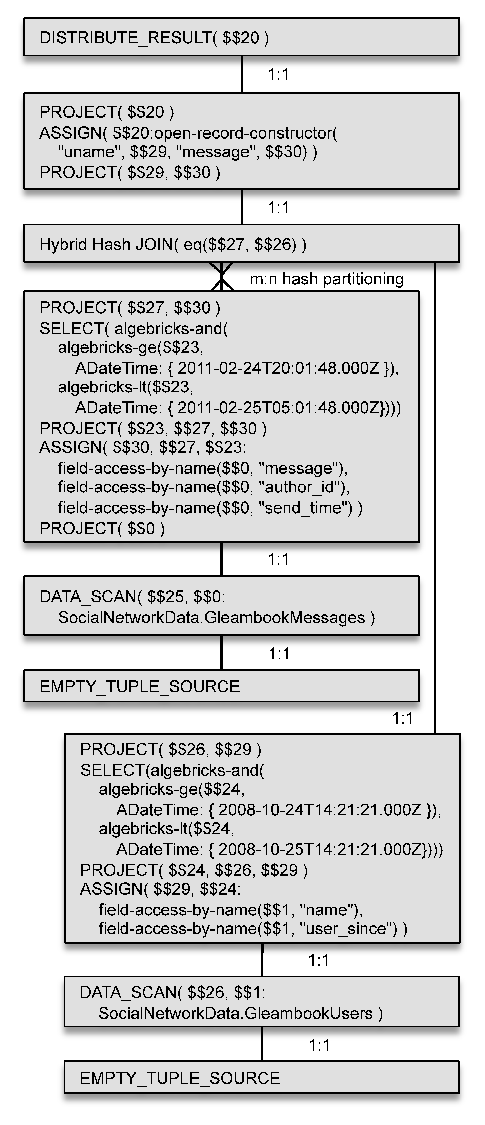
\includegraphics[width=0.5\columnwidth]{images/asterix_hyracks_job_renamed}
\vspace{-1ex}
\caption{AsterixDB Hyracks Job.}
\vspace{-.8ex}
\label{fig:asterix_hyracks_job}
\end{figure}

Then, the Algebricks optimizer transforms the initial logical plan into an optimized physical plan by applying logical and physical rewriting rules.
The optimizer utilizes 48 AsterixDB specific rules and 41 generic Algebricks rules. 
Figure~\ref{fig:asterix_hyracks_job} visualizes the generated Hyracks job for this example query.

Note that the final optimized Hyracks job has the following main differences from the original plan:

\begin{list}{\labelitemi}{\leftmargin=1em}\itemsep 0pt \parskip 0pt

\item A hybrid hash join operator is introduced to evaluate
the equality join condition.

\item The original select conditions are pushed into the two join branches.

\item Project operators are injected into the plan wherever necessary.

\item A hash partition exchange operator is enforced for the ``GleambookMessages'' branch to make sure data from this branch is partitioned by ``author\_id''.  Note that there is no re-partition exchange for the ``GleambookUsers'' branch because data from this branch has already been hash partitioned across the cluster according to the primary key ``id''.

\end{list}



\eat{
\begin{center}
\scriptsize
\begin{lstlisting}
DISTRIBUTE_RESULT( $$20 )
ONE_TO_ONE_EXCHANGE
PROJECT( $$20 )
ASSIGN( $$20:closed-record-constructor(
    "uname", $$29, "message", $$30) )
PROJECT( $$29, $$30 )
ONE_TO_ONE_EXCHANGE
Hybrid Hash JOIN( algebricks-eq($$27, $$26) )
{
  HASH_PARTITION_EXCHANGE( $$27 )
  PROJECT( $$27, $$30 )
  SELECT( algebricks-and(
      algebricks-ge($$23,
          ADateTime: { 2011-02-24T20:01:48.000Z }),
      algebricks-lt($$23, 
          ADateTime: { 2011-02-25T05:01:48.000Z })) )
  PROJECT( $$23, $$27, $$30 )
  ASSIGN( $$30, $$27, $$23:
      field-access-by-index($$0, 6), 
      field-access-by-index($$0, 2), 
      field-access-by-index($$0, 5) )
  PROJECT( $$0 )
  ONE_TO_ONE_EXCHANGE
  DATA_SCAN( $$25, $$0:demo.FacebookMessages )
  ONE_TO_ONE_EXCHANGE
  EMPTY_TUPLE_SOURCE
} {
  ONE_TO_ONE_EXCHANGE
  PROJECT( $$26, $$29 )
  SELECT( algebricks-and(
      algebricks-ge($$24,
          ADateTime: { 2008-10-24T14:21:21.000Z }), 
      algebricks-lt($$24, 
          ADateTime: { 2008-10-25T14:21:21.000Z })) )
  PROJECT( $$24, $$26, $$29 )
  ASSIGN( $$29, $$24:
      field-access-by-index($$1, 3), 
      field-access-by-index($$1, 5) )
  ONE_TO_ONE_EXCHANGE
  DATA_SCAN( $$26, $$1:demo.FacebookUsers )
  ONE_TO_ONE_EXCHANGE
  EMPTY_TUPLE_SOURCE
}
\end{lstlisting}
\end{center}
}


\subsection{Apache VXQuery}

\eat{
Highlights
\begin{itemize}

  \item path step optimizations
  \item xquery logic vs algebricks logic
  \item XML parser 
  \item query plan includes type information
\end{itemize}
}

Apache VXQuery is an XQuery processor built for handling large collections of XML data. 
It uses Algebricks and Hyracks to process XML by adding a binary representation of the XQuery Data Model (XDM), an XQuery parser, an XQuery optimizer, and the data model dependent expressions.
VXQuery is intended to implement the complete XQuery specification.

The example XQuery statement is based on weather data provided by the NOAA \cite{NOAA-GHCND:website}.
The query finds all precipitation ("PRCP") records for the "GHCND:USW00014771" station that occurred during 1999.
The precipitation readings are recorded in tenths of an inch.
After summing all readings, the result is divided by 10 to find the total precipitation for 1999 in inches.
The query (also included in our experiments as VQ2) is shown below followed by a sample XML weather record:

\lstset{numbers=left, numberstyle=\tiny, stepnumber=1, numbersep=5pt}
\begin{center}
\scriptsize
\begin{lstlisting}
fn:sum(
  for $r in collection("sensors")/dataCollection/data
  where $r/station eq "GHCND:USW00014771" 
    and $r/dataType eq "PRCP" 
    and year-from-dateTime(xs:dateTime(data($r/date))) 
        eq 1999
  return $r/value
) div 10
\end{lstlisting}
\end{center}

\lstset{numbers=left, numberstyle=\tiny, stepnumber=1, numbersep=5pt}
\begin{center}
\scriptsize
\begin{lstlisting}
<?xml version="1.0" encoding="UTF-8" standalone="yes"?>
<dataCollection pageCount="1" totalCount="3">
  <data>
    <date>1999-12-02T00:00:00.000</date>
    <dataType>PRCP</dataType>
    <station>GHCND:USW00014771</station>
    <value>0</value>
    <attributes>
      <attribute></attribute>
      <attribute></attribute>
      <attribute>a</attribute>
      <attribute></attribute>
    </attributes>
  </data>
  <data>
    <date>1999-12-02T00:00:00.000</date>
    <dataType>TMIN</dataType>
    <station>GHCND:USW00014771</station>
    <value>-6</value>
    <attributes>
      <attribute></attribute>
      <attribute></attribute>
      <attribute>0</attribute>
      <attribute></attribute>
    </attributes>
  </data>
</dataCollection>
\end{lstlisting}
\end{center}

Apache VXQuery begins by translating the XQuery statement into a logical query plan using the Algebricks logical operators.
The translator follows the XQuery specification and creates a correct Algebricks query plan with all the XQuery type checking expressions translated into the query plan.
The optimizer will use these expressions to type check the query plan.
%\yingyi{Prestion, is type checking done here?  It seems different
%from what we discussed.}.
%The translator takes a strict approach to building a logical query plan.
%The plan includes all the necessary type checking for data flowing through the query.

XQuery is a complex language with well-defined but complicated semantics for various parts of the language~\cite{XQuery-W3C-Formal-Semantics}.
Below we show the initial Algebricks logical plan generated by the VXQuery translator for the weather query.
Note that what appears as a simple path-step in XQuery (the / operator), is equivalent to a more complex expression that involves unnesting, sorting, duplicate-elimination, etc.
For example, lines 68-74 in the listing below represent "/dataCollection".
Please note that while we do not expect the reader to glean all the details of the plan shown, we wish to communicate the fact that Algebricks is capable of implementing the semantics of a complex query language like XQuery.

\newpage

%\definecolor{light-gray}{gray}{0.80}

\lstset{numbers=left, numberstyle=\tiny, stepnumber=1, numbersep=5pt}
\begin{center}
\scriptsize
\begin{lstlisting}
DISTRIBUTE-RESULT( $$59 )
UNNEST( $$59:iterate($$58) )
ASSIGN( $$58:divide(promote(<anyAtomicType?>, data($$56)), 
    promote(<anyAtomicType?>, data($$57))) )
ASSIGN( $$57:10 )
ASSIGN( $$56:sum(promote(<anyAtomicType*>, data($$55))) )
SUBPLAN {
  AGGREGATE( $$55:sequence($$54) )
  ASSIGN( $$54:sort-distinct-nodes-asc-or-atomics($$53) )
  SUBPLAN {
    AGGREGATE( $$53:sequence(child("value", 
        treat(<node*>, $$51))) )
    UNNEST( $$51:iterate($$49)
    NESTED-TUPLE-SOURCE
  }
  ASSIGN( $$49:treat(<item>, $$19) )
  SELECT( boolean($$48) )
  ASSIGN( $$48:and(boolean(data($$36)), 
      boolean(data($$47))) )
  ASSIGN( $$47:value-eq(promote(<anyAtomicType?>, 
      data($$45)), promote(<anyAtomicType?>,data($$46))) )
  ASSIGN( $$46:1999 )
  ASSIGN( $$45:year-from-dateTime(promote(<dateTime?>, 
      data($$44))) )
  ASSIGN( $$44:cast(<dateTime?>, $$43) )
  ASSIGN( $$43:data(treat(<item*>, $$42)) )
  ASSIGN( $$42:sort-distinct-nodes-asc-or-atomics($$41) )
  SUBPLAN {
    AGGREGATE( $$41:sequence(child("date", 
        treat(<node*>, $$39))) )
    UNNEST( $$39:iterate($$37) )
    NESTED-TUPLE-SOURCE
  }
  ASSIGN( $$37:treat(<item>, $$19) )
  ASSIGN( $$36:and(boolean(data($$27)), 
      boolean(data($$35))) )
  ASSIGN( $$35:value-eq(promote(<anyAtomicType?>, 
      data($$33)), promote(<anyAtomicType?>,data($$34))) )
  ASSIGN( $$34:"PRCP" )
  ASSIGN( $$33:sort-distinct-nodes-asc-or-atomics($$32))
  SUBPLAN {
    AGGREGATE( $$32:sequence(child("dataType", 
        treat(<node*>, $$30))) )
    UNNEST( $$30:iterate($$28) )
    NESTED-TUPLE-SOURCE
  }
  ASSIGN( $$28:treat(<item>, $$19) )
  ASSIGN( $$27:value-eq(promote(<anyAtomicType?>, 
      data($$25)),promote(<anyAtomicType?>,data($$26)) ) )
  ASSIGN( $$26:"GHCND:USW00014771" )
  ASSIGN( $$25:sort-distinct-nodes-asc-or-atomics($$24) )
  SUBPLAN {
    AGGREGATE( $$24:sequence(child("station", 
        treat(<node*>, $$22))) )
    UNNEST( $$22:iterate($$20) )
    NESTED-TUPLE-SOURCE
  }
  ASSIGN( $$20:treat(<item>, $$19) )
  UNNEST( $$19:iterate($$18) )
  ASSIGN( $$18:sort-distinct-nodes-asc-or-atomics($$17) )
  SUBPLAN {
    AGGREGATE( $$17:sequence(child("data", 
        treat(<node*>, $$15))) )
    UNNEST( $$15:iterate($$13) )
    ASSIGN( $$13:sort-distinct-nodes-asc-or-atomics($$12))
    NESTED-TUPLE-SOURCE
  }
  SUBPLAN {
    AGGREGATE( $$12:sequence(child("dataCollection", 
        treat(<node*>, $$10))) )
    UNNEST( $$10:iterate($$8) )
    ASSIGN( $$8:sort-distinct-nodes-asc-or-atomics($$7) )
    NESTED-TUPLE-SOURCE
  }
  SUBPLAN {
    AGGREGATE( $$7:sequence(child("root", 
        treat(<node*>, $$5))) )
    UNNEST( $$5:iterate($$3) )
    NESTED-TUPLE-SOURCE
  }
  ASSIGN( $$3:collection(promote(<string>, data($$2))) )
  ASSIGN( $$2:treat(<item>, $$1) )
  ASSIGN( $$1:"/sensors" )
  NESTED-TUPLE-SOURCE
}
EMPTY-TUPLE-SOURCE
\end{lstlisting}
\end{center}

After translating the plan, the Algebricks query optimization phase uses 22 Apache VXQuery rules and 30 generic Algebricks rules to create an optimized logical plan.
Apache VXQuery rules apply basic XQuery data type rules and path step expression optimizations to streamline the plan.
One of Algebricks' benefits to this plan is a more efficient way to calculate the aggregation.
Using Algebricks logical operators, the built-in rules enable efficient two-step aggregation across the cluster.
Further, the VXQuery query optimizer provides data specific details - enabling parallelization of the query plan.
Apache VXQuery achieves parallel execution simply by providing XQuery function properties to Algebricks. 
%Since XQuery's logical expressions use trinary logic, the Algebricks logic expressions are only used for optimizing when the XQuery expression is matched with a boolean effective value expresion ("boolean").
%The optimized query plan is show below:

In the job generation phase, the VXQuery Metadata Interface implementation finds how the non-fragmented XML documents are partitioned throughout a cluster.
Each machine has a unique set of XML documents residing in a directory specified by the query's fn:doc or fn:collection function.
While AsterixDB has a native storage option, Apache VXQuery scans external XML documents for each query.
The weather query uses the collection function to identify the ``sensors" directory on all nodes.
Using the plan and the metadata interface, Algebricks creates the Hyracks job shown in Figure \ref{fig:vxquery_hyracks_job}.

\begin{figure}[tb]
\vspace{-.8ex}
\centering
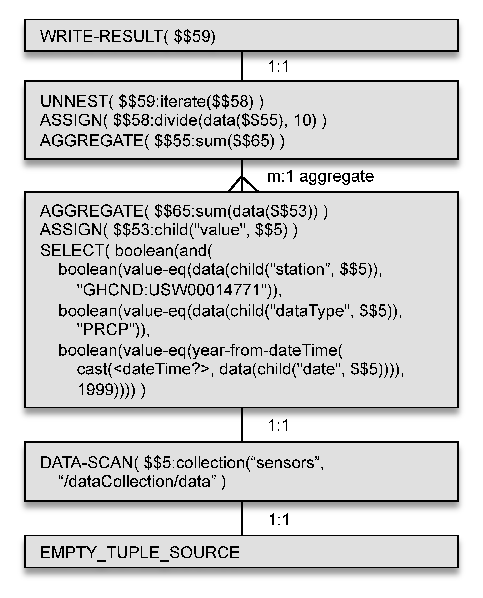
\includegraphics[width=0.50\columnwidth]{images/vxquery_hyracks_job}
\vspace{-1ex}
\caption{VXQuery Hyracks Job.}
\vspace{-.8ex}
\label{fig:vxquery_hyracks_job}
\end{figure}

\eat{
\begin{center}
\scriptsize
\begin{lstlisting}
DISTRIBUTE-RESULT ( $$59 )
ONE_TO_ONE_EXCHANGE
UNNEST( $$59:iterate($$58) )
ASSIGN( $$58:divide(data($$55), 10) )
AGGREGATE( $$55:sum($$65) )
RANDOM_MERGE_EXCHANGE
AGGREGATE( $$65:sum(data($$53)) )
ASSIGN( $$53:child("value", $$5) )
SELECT( boolean(and(
    boolean(value-eq(data(child("station", $$5)), 
        "GHCND:USW00014771")), 
    boolean(value-eq(data(child("dataType", $$5)), 
        "PRCP")), 
    boolean(value-eq(year-from-dateTime(cast(<dateTime?>, 
        data(child("date", $$5)))), 1999)))) )
ONE_TO_ONE_EXCHANGE
DATA-SCAN( $$5:collection("sensors", 
    "/dataCollection/data") )
ONE_TO_ONE_EXCHANGE
EMPTY-TUPLE-SOURCE
\end{lstlisting}
\end{center}
}

In the current implementation of VXQuery, we assume a collection of many (typically small) XML files. Nevertheless, Algebricks can also handle parallelization of queries over a single large document stored on a distributed storage system such as HDFS. We are currently implementing a parallel XML parser similar to \cite{oracle:xquery:website} to enable these use cases.
%Finally, Apache VXQuery can efficiently handle the query as long as each descendant tag node fits into the available memory.

\eat{
% Looks like this is covered inline for VXQuery
Note the following Apache VXQuery optimizations for the logical plan:

\begin{list}{\labelitemi}{\leftmargin=1em}\itemsep 0pt \parskip 0pt

\item The path step expression have been merged into the DATA-SCAN operator. As a result only the designated element is added to the data flow.

\item The aggregation is done using a local node sum and then a global sum from each node.

\item The SELECT operator's conditional expression has been inlined.

\end{list}
}


%The Metadata Interface specifies the XQuery parser, a SAX based XML parser, to read and translate the XML documents into XQuery Data Model (XDM) instances.
\eat{
The query demonstrates how Algebricks supports aggregation in multiple query languages.
In addition, Algebricks provides a framework to implement language specific optimizations: for example, XQuery has optimized the path step expression using Algebricks rewrite rules.
}

\section{Experimental Evaluation}\label{sec:experiments}

In this section, we demonstrate experimentally the parallel efficiency of Hivesterix, AsterixDB, and VXQuery. In addition to showing proof of their existence, these experiments aim to expose the direct benefits of using Algebricks in achieving good parallelization characteristics. We report performance for a representative set of queries for each system for different sizes of data and different numbers of nodes, with the goal of showing the scale-up and speed-up characteristics of each system.

\subsection{Hivesterix}
\noindent\textbf{Cluster}: We ran Hivesterix experiments on a 40-node cluster with a Gigabit Ethernet switch. 
Each node had a Quadcore Intel Xeon CPU E3-1230 V2 3.30GHz, 16GB of RAM, and 3TB RAID0 (3x1TB disks, linux software RAID). We compared Hivesterix and Hive-on-Hadoop (Hive-0.12.0). In the experiments,
the RAID0 disk on each node is used for the HDFS data directory
and the spilling workspace for query processing.
\noindent\textbf{Data}: For speedup experiments, we used TPC-H 250$\times$ (~250GB). For scaleup experiments, we used TPC-H 250$\times$,
500$\times$, 750$\times$, 1000$\times$ (~1TB) for 10, 20,
30, and 40 machines respectively.
\noindent\textbf{Configuration}: We ran eight partitions per machine.
\noindent\textbf{Queries}: We report three representative queries
from the TPC-H benchmark, a filter and aggregate query, a group-by query, and 
a join with group-by query, shown below.

\subsubsection*{HQ1: Filter + Aggregate Query (TPC-H Q14)}

\begin{lstlisting}
select sum(l_extendedprice*l_discount) as revenue
from lineitem
where l_shipdate >= '1994-01-01'
  and l_shipdate < '1995-01-01'
  and l_discount >= 0.05 and l_discount <= 0.07
  and l_quantity < 24;
\end{lstlisting}

\subsubsection*{HQ2: Group-by Query (TPC-H Q1)}

\begin{lstlisting}
select l_returnflag, l_linestatus, sum(l_quantity), 
  sum(l_extendedprice), 
  sum(l_extendedprice*(1-l_discount)),     
  sum(l_extendedprice*(1-l_discount)*(1+l_tax)), 
  avg(l_quantity), avg(l_extendedprice), avg(l_discount), 
  count(1) 
from lineitem 
where l_shipdate <= '1998-09-02' 
group by l_returnflag, l_linestatus 
order by l_returnflag, l_linestatus;
\end{lstlisting}

\subsubsection*{HQ3: Join + Group-By Query (TPC-H Q9)}

\begin{lstlisting}
select nation, o_year, sum(amount) as sum_profit
from (
  select n_name as nation, year(o_orderdate) as o_year, 
    l_extendedprice * (1 - l_discount) -  
    ps_supplycost * l_quantity as amount
  from orders o join (
    select l_extendedprice, l_discount, l_quantity, 
      l_orderkey, n_name, ps_supplycost 
    from part p join (
      select l_extendedprice, l_discount, l_quantity, 
        l_partkey, l_orderkey, n_name, ps_supplycost 
      from partsupp ps join (
        select l_suppkey, l_extendedprice, l_discount, 
          l_quantity, l_partkey, l_orderkey, n_name 
        from (
          select s_suppkey, n_name 
          from nation n join supplier s 
            on n.n_nationkey = s.s_nationkey
        ) s1 join lineitem l on s1.s_suppkey = l.l_suppkey
      ) l1 on ps.ps_suppkey = l1.l_suppkey 
          and ps.ps_partkey = l1.l_partkey
    ) l2 on p.p_name like '%green%' 
        and p.p_partkey = l2.l_partkey
  ) l3 on o.o_orderkey = l3.l_orderkey
) profit
group by nation, o_year
order by nation, o_year desc;
\end{lstlisting}

As indicated by Figures~\ref{fig:hivestrix_speed_up} and~\ref{fig:hivestrix_scale_up}, all queries show good speed-up and scale-up characteristics. All three benefit from scanning blocks of HDFS data in parallel. In HQ1 and HQ2, filtering is parallelized and aggregation is done in two phases, reducing the amount of data transferred across machines. HQ3 benefits from parallelizing joins across the cluster.
We have also executed TPC-H using Hive-on-Hadoop (Hive-0.12.0) and
a comparison with Hivesterix is shown in 
Figure~\ref{fig:hivestrix_hive}. (An interesting future exercise might include the new generation of "SQL on Hadoop" systems.)

\begin{figure}[!ht]
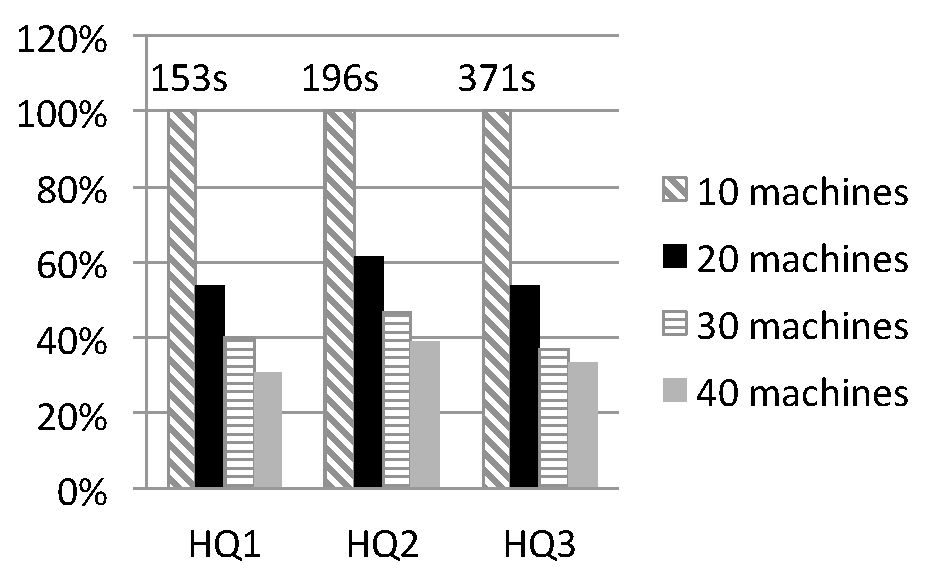
\includegraphics[width=\columnfigurewidth]{images/hivestrix_speed_up}
\centering
\vspace{-2ex}
\caption{Hivesterix cluster speed up (percentage of 10 machines).}
\label{fig:hivestrix_speed_up}
\end{figure}

\begin{figure}[!ht]
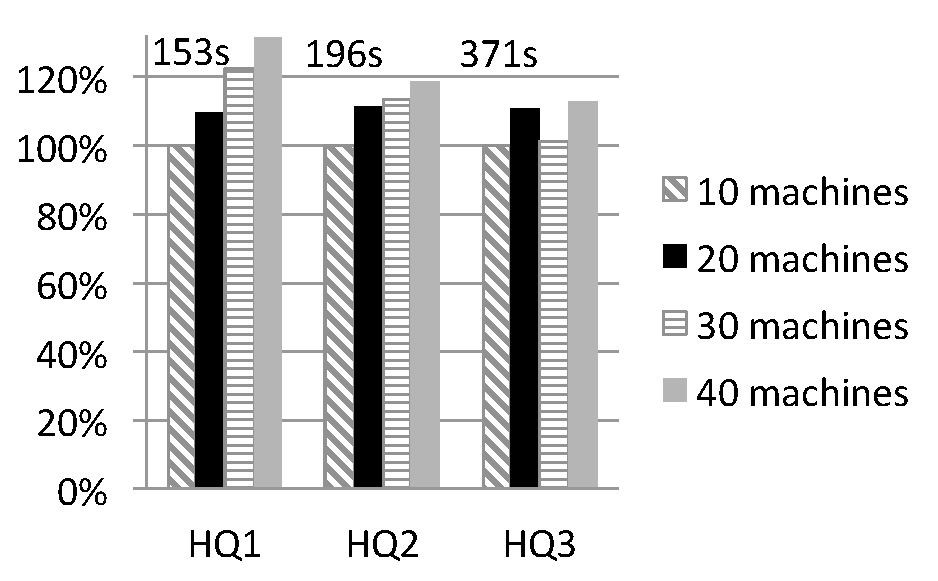
\includegraphics[width=\columnfigurewidth]{images/hivestrix_scale_up}
\centering
\vspace{-2ex}
\caption{Hivesterix cluster scale up (percentage of 10 machines).}
\label{fig:hivestrix_scale_up}
\end{figure}

\begin{figure}[!ht]
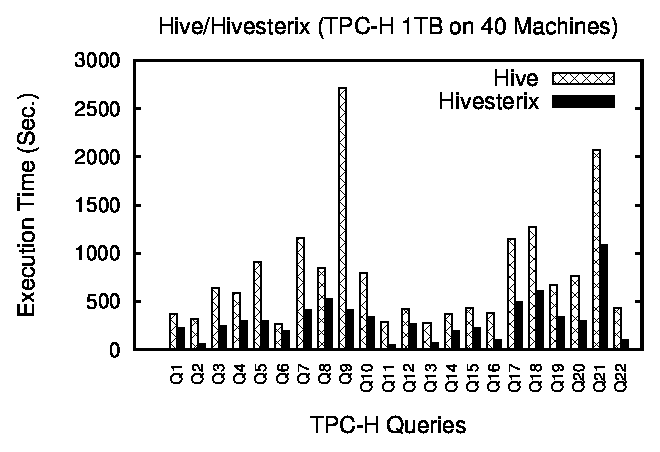
\includegraphics[width=\columnfigurewidth]{images/hivesterix}
\centering
\vspace{-1ex}
\caption{Hivesterix and Hive-on-Hadoop Comparison on TPC-H.}
\label{fig:hivestrix_hive}
\end{figure}


\subsection{Apache AsterixDB}

\eat{
\begin{itemize}
\item Asterix cluster description.
\item Show \& briefly describe each query.
\item Emphasize on the fact that the queries belong to different categories, and there is a huge difference in their running time (they do operations with naturally different costs and may exploit an index (as it exists in AsterixDB) which can change the data access path and performance considerably).
\item Present and explain Scale-up and Speed-up graphs separately.
\end{itemize}
}

\noindent\textbf{Cluster}: We ran the reported experiments on a 10-node IBM x3650 cluster with a Gigabit Ethernet switch. Each node had one Intel Xeon processor E5520 2.26GHz with four cores, 12GB of RAM, and four 300GB, 10K RPM hard disks. On each machine 3 disks were used for data. The other disk was used to store "system's data" (transaction logs and system logs).
\noindent\textbf{Data}: We used a synthetic data generator to create records for the collections related to these tests (``GleambookUsers'' etc.) For the speedup experiments, we generated 338GB of data, loaded on 9, 18 and 27 partitions. For the scaleup experiments, we generated 169GB, 338GB and 507GB of data for 9, 18 and 27 partitions respectively. A secondary index was constructed on the user\_since field of the GleambookUsers dataset.
%\yingyi{Pouria, can you please add the data description like that in the Hivesterix subsection?}
\noindent\textbf{Configuration}: We ran three partitions on each machine. 
We assigned a maximum of 6GB of memory to each node controller. 
The buffercache size for each node controller was set to be 1GB.
%\yingyi{Pouria, can you please add the configuration description like that in the Hivesterix subsection?}
\noindent\textbf{Queries}: We executed four representative AQL queries, as follows.

\subsubsection*{AQ1: Filter Query}

\begin{lstlisting}
for $t in dataset GleambookMessages
where $t.author_id < 0
return $t
\end{lstlisting}


\subsubsection*{AQ2: Filter Query Using Indexes}

\begin{lstlisting}
for $user in dataset GleambookUsers
where $user.user_since >= datetime('2005-08-16T15:52:14') 
and $user.user_since < datetime('2005-08-16T15:57:14') 
return $user
\end{lstlisting}



\subsubsection*{AQ3: Aggregate Query}

\begin{lstlisting}
avg(
  for $t in dataset ChirpMessages
  where $t.send_time >= datetime('2008-11-15T19:42:51')  
    and $t.send_time < datetime('2008-11-15T23:27:51')  
  return string-length($t.message_text)
)
\end{lstlisting}



\subsubsection*{AQ4: Join Query}

\begin{lstlisting}
for $message in dataset GleambookMessages
for $user in dataset GleambookUsers
where $message.author_id = $user.id 
  and $user.user_since >= datetime('2011-02-24T20:01:48')
  and $user.user_since < datetime('2011-02-25T05:01:48')
  and $message.send_time >=datetime('2008-10-24T14:21:21')
  and $message.send_time < datetime('2008-10-25T14:21:21')
return {
  "uname": $user.name,
  "message": $message.message
}
\end{lstlisting}


% Numbers can be found in the Google spread sheet.

\begin{figure}[tb]
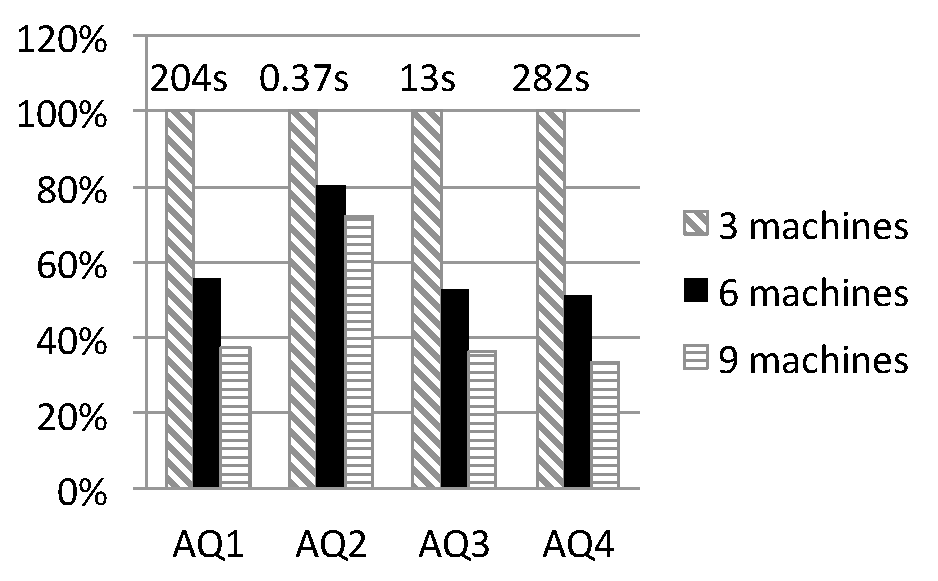
\includegraphics[width=\columnfigurewidth]{images/asterix_speed_up}
\centering
\vspace{-2ex}
\caption{AsterixDB cluster speed up (percentage of 3 machines).}
\label{fig:asterixdb_speed_up}
\end{figure}

\begin{figure}[tb]
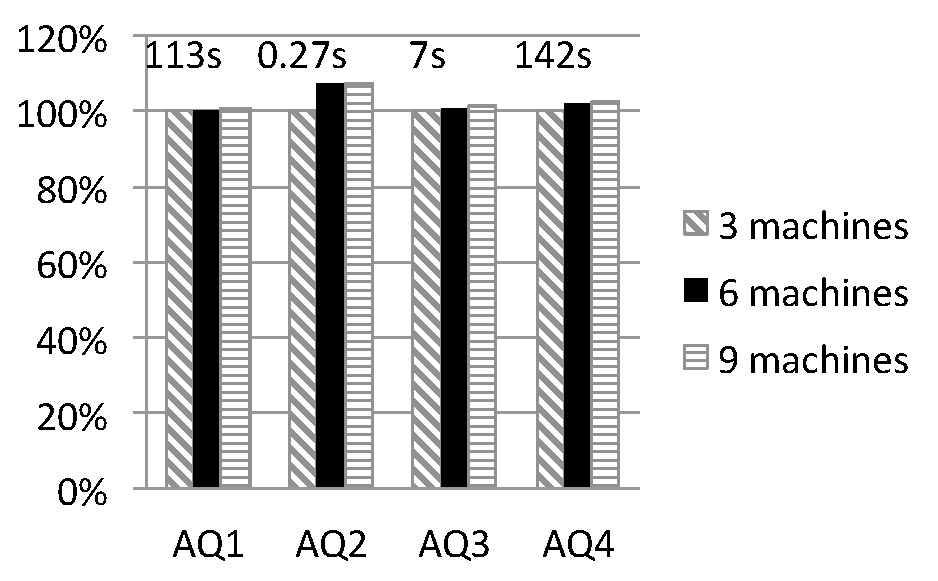
\includegraphics[width=\columnfigurewidth]{images/asterix_scale_up}
\centering
\vspace{-2ex}
\caption{AsterixDB cluster scale up (percentage of 3 machines).}
%\vspace{-3ex}
\label{fig:asterixdb_scale_up}
\end{figure}

Figure~\ref{fig:asterixdb_speed_up} and Figure~\ref{fig:asterixdb_scale_up} depict the parallel speedup and scaleup of the four AQL queries. AQ1 and AQ3 benefit from the same rules in Algebricks that helped HQ1 and HQ2 in Hivesterix. Scanning partitions and filtering is done in parallel on the different nodes of the cluster. In AQ3, the aggregation is performed in two phases to reduce network transfer. Join parallelism allows AQ4 to use the cluster effectively. AQ2 uses an index in AsterixDB to evaluate filters instead of scanning all the data. The index range scan is performed in parallel on the different partitions. Note that Algebricks includes facilities for utilizing indexes for query processing, but AsterixDB is currently the only system built on top of Algebricks that implements indexing at the storage level.
Detailed AsterixDB performance characteristics can be found in~\cite{ASTERIX}.



\subsection{Apache VXQuery}\label{sec:VXQuery}

\eat{
Highlights
\begin{itemize}

  \item XML parsing dominates query time 
  \item real weather data

\end{itemize}
}

\noindent \textbf{Cluster}: Experiments were run on a cluster whose nodes have two Dual-Core AMD Opteron(tm) processor 2212 HE CPUs, 8GB of RAM, and two 1TB hard drives. 
\noindent \textbf{Data}: We used NOAA's Global Historical Climatology Network (GHCN)-Daily dataset that includes daily summaries of climate recordings (e.g., high and low temperatures, wind speed, rainfall). 
The complete XML data definition can be found on NOAA's site \cite{NOAA-GHCND:website}. 
For the speed-up experiments, we used 57GB of weather  XML data partitioned over the number of machines (varied from 1 to 8) for each run.
The scale-up experiments were performed while keeping the amount of data per machine constant at 7.2GB and varying the number of machines from 1 to 8. 
%for each of the queries shown below.
\noindent \textbf{Configuration}: We ran four partitions per machine.
\noindent \textbf{Queries}: We used the following three XQuery queries:

\subsubsection*{VQ1: Filter Query}\label{query:VQ1}
% VQ1 represents VXQuery's benchmark query Q01
Query VQ1 filters the data to show all readings that report an extreme wind warning. 
Such warnings occur when the wind speed exceeds 110 mph. 
(The wind measurement unit, tenths of a meter per second, has been converted to miles per hour.)

\begin{lstlisting}
for $r in collection("sensors")/dataCollection/data
where $r/dataType eq "AWND"
  and xs:decimal(data($r/value)) gt 491.744
return $r
\end{lstlisting}


\subsubsection*{VQ2: Aggregate Query}\label{query:VQ2}
% VQ2 represents VXQuery's benchmark query Q02
Query VQ2 finds the annual precipitation for Syracuse, NY using the airport weather station (USW00014771) for 1999. 
The precipitation is reported in tenths of an inch. 

\begin{lstlisting}
sum(
  for $r in collection("sensors")/dataCollection/data
  where $r/station eq "GHCND:USW00014771" 
    and $r/dataType eq "PRCP" 
    and year-from-dateTime(xs:dateTime(data($r/date))) 
        eq 1999
  return $r/value
) div 10
\end{lstlisting}



\subsubsection*{VQ3: Join + Aggregate Query}\label{query:VQ3}
% VQ3 represents VXQuery's benchmark query Q05
Query VQ3 finds the lowest recorded temperature (TMIN) in the United States for 2001. 
This query includes nested loops which are commonly used in XQuery.
While XQuery does not have a join expression, these nested loops can be converted into a join operation using the Algebricks join operator.
Converting a nested loop into a more efficient join algorithm provides the expected performance improvement for Apache VXQuery.
%with a speed improvement over naive implementations. 


\begin{lstlisting}
min(
  for $s in 
      collection("stations")/stationCollection/station
  for $r in collection("sensors")/dataCollection/data
  where $s/id eq $r/station
    and (some $x in $s/locationLabels satisfies 
        ($x/type eq "CNTRY" and $x/id eq "FIPS:US"))
    and $r/dataType eq "TMIN" 
    and year-from-dateTime(xs:dateTime(data($r/date))) 
        eq 2001
  return $r/value
) div 10
\end{lstlisting}


% Numbers can be found in the Google spread sheet.

\begin{figure}[tb]
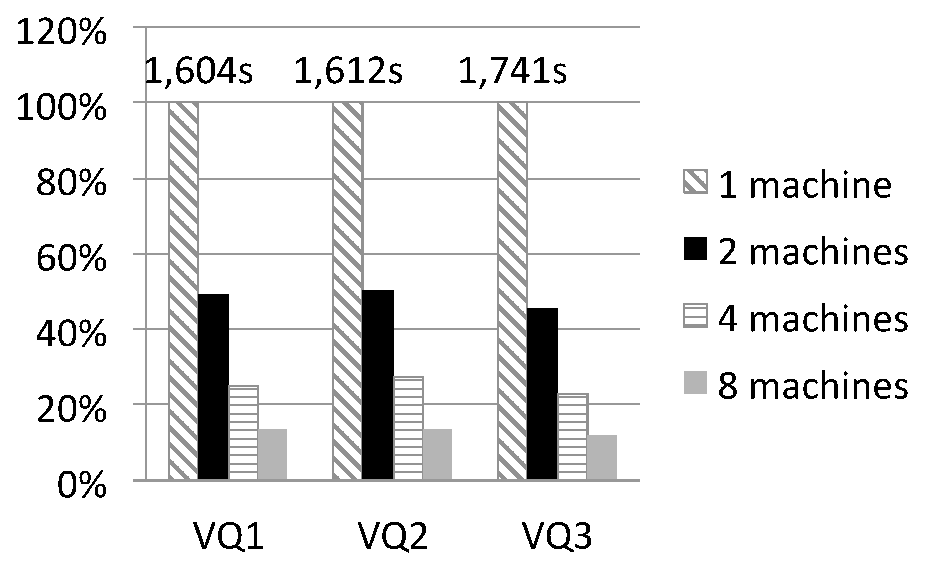
\includegraphics[width=\columnfigurewidth]{images/vxquery_speed_up}
\centering
\vspace{-2ex}
\caption{VXQuery cluster speed up (percentage of 1 machine).}
%\vspace{-1ex}
\label{fig:vxquery_speed_up}
\end{figure}

\begin{figure}[tb]
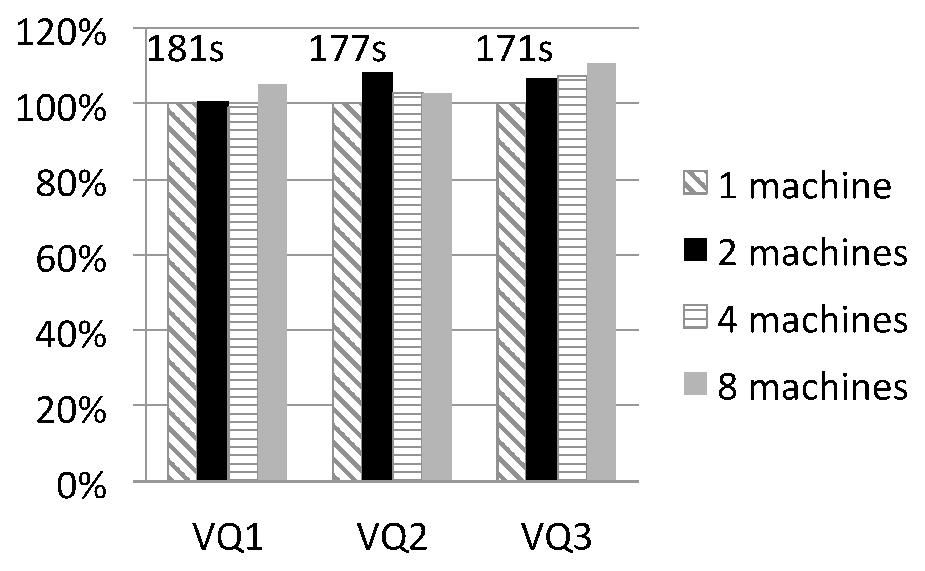
\includegraphics[width=\columnfigurewidth]{images/vxquery_scale_up}
\centering
\vspace{-2ex}
\caption{VXQuery cluster scale up (percentage of 1 machine).}
%\vspace{-1ex}
\label{fig:vxquery_scale_up}
\end{figure}

Figure~\ref{fig:vxquery_speed_up} and Figure~\ref{fig:vxquery_scale_up} show the parallel speedup and scaleup of Apache VXQuery. The optimizations implemented in Algebricks help VQ1, VQ2, and VQ3 to achieve good parallel performance by parallelizing scans, filters, aggregations, and joins.
More performance results for the current Apache VXQuery implementation on top of Algebricks can be found in \cite{Carman:2015}.

\section{Conclusion}

Algebricks has served as a useful tool to build not just the AsterixDB query compiler, but also query compilers for HiveQL and XQuery. Table~\ref{tbl:codemetrics} shows the lines of code, the number of rewrite rules, the number of logical operators, and the number of physical operators that were provided by Algebricks, and those that needed to be additionally implemented in AsterixDB, Hivesterix, and VXQuery. Algebricks provides about 50 rewrite rules, 39 logical operators, and 44 physical operators that are helpful for all three query processors. Additionally, AsterixDB required only 2 logical operators and 6 physical operators. These operators were AsterixDB specific and related to accessing indexes. The extensibility offered by Algebricks allowed the AsterixDB platform to implement these operators and plug them into the Algebricks framework. 61 rewrite rules were implemented in the AsterixDB platform to deal with rewrites specific to the Asterix data model. Hivesterix and VXQuery did not require any additional operators. Operators available in Algebricks were sufficient to implement the entire HiveQL and XQuery language compilers. Hivesterix and VXQuery required 4 and 29 rewrite rules, respectively, that were specific to the datamodel semantics of the two systems.


\begin{table}
\begin{center}
\begin{tabular}{|l|l|l|l|l|}
\hline
 & Algebricks & AsterixDB & Hivesterix & VXQuery \\
\hline
\hline
LOC & 42K & 40K & 3.4K & 12.8K \\
\hline
\# Rules & 50 & 61 & 4 & 29 \\
\hline
\# Logical Ops & 39 & 2 & 0 & 0 \\
\hline
\# Physical Ops & 44 & 6 & 0 & 0 \\
\hline
\end{tabular}
\caption{Code metrics as a proxy for the effort required to build query compilers using Algebricks}\label{tbl:codemetrics}
\end{center}
\end{table}

In the next chapter, we look more in detail at how Algebricks was used in implementing the query processing layer of AsterixDB.
